 \documentclass[a4paper,journal]{IEEEtran}

\usepackage{cite}
\usepackage[utf8]{inputenc}
\usepackage{graphicx}
\usepackage{float}
\usepackage{color, colortbl}
\usepackage{xcolor}
\usepackage{array}
\usepackage{multirow}
\usepackage{footnote}
\usepackage{cite}
%The below is used to add notes to tables without disrupting the IEEEtran format
\usepackage[normal]{threeparttable}
%Multiple figures in a row
%\usepackage{caption}
%\usepackage{subcaption}
\usepackage{amsmath}
\usepackage{mathtools}

%Put the references in a nice way so the empty space is not overly great.
%\usepackage{flushend}

%Algorithms
\usepackage[linesnumbered,vlined,norelsize]{algorithm2e}

%\usepackage[hyphens]{url}
\usepackage{caption}
\usepackage{subcaption}

\usepackage{hyperref}
% Disable below if wanting to comply exclusively to conference mode of IEEEtran
% \IEEEoverridecommandlockouts

%ommit the error about the algorithm
\makeatletter
\newcommand{\removelatexerror}{\let\@latex@error\@gobble}
\makeatother

%put a footnote without number
\makeatletter
\def\blfootnote{\xdef\@thefnmark{}\@footnotetext}
\makeatother

\usepackage{lipsum}

\newcommand{\FGC}[1]{\textcolor{blue} {({\bf COMMENT: }#1)}}
\newcommand{\FGT}[1]{\textcolor{red} {#1}}

\title{Traffic Differentiation in Dense Collision-free WLANs}
  %\author{Luis Sanabria-Russo and Francesco Gringoli
%	\author{\IEEEauthorblockN{Luis Sanabria-Russo\IEEEauthorrefmark{3}}\\
     \author{\IEEEauthorblockN{Luis Sanabria-Russo\IEEEauthorrefmark{0}, Boris Bellalta\IEEEauthorrefmark{0}}\\
      \IEEEauthorblockA{\IEEEauthorrefmark{0}Department of Information and Communication Technologies \\ Universitat Pompeu Fabra, Barcelona, Spain
      \\\ {\tt \{luis.sanabria,boris.bellalta\}@upf.edu}}\\
     % \IEEEauthorblockA{\IEEEauthorrefmark{2}CNIT / University of Brescia, Brescia, Italy
%      \\\ {\tt francesco.gringoli@ing.unibs.it}}
  }


\begin{document}

%\date{\today}
\maketitle

\begin{abstract}
The ability to perform traffic differentiation is a promising feature of the current Medium Access Control (MAC) in Wireless Local Area Networks (WLANs). The Enhaced Distributed Channel Access (EDCA) MAC protocol for WLANs proposes up to four Access Categories (AC) that can be mapped to different traffic priorities. High priority ACs are allowed to transmit more often that low priority AC, providing a way of prioritizing delay sensitive traffic like voice calls or video streaming. Further, EDCA also considers the intricacies related to the management of multiple queues, virtual collisions and priority. Carrier Sense Multiple Access with Enhanced Collision Avoidance (CSMA/ECA) is a compatible MAC protocol for WLANs which is also capable of providing traffic differentiation. Contrary to EDCA, CSMA/ECA uses a deterministic backoff technique which is capable of constructing collision-free schedules for each AC. This work proposes traffic differentiation with CSMA/ECA for the first time. It describes the mechanisms used by CSMA/ECA to construct collision-free schedules with multiple queues, avoid Virtual Collisions (VC) and present simulation results that show CSMA/ECA outperforming EDCA in different commonly-found networking scenarios.
\end{abstract}

\begin{IEEEkeywords}
Wireless LAN, Multiaccess Communication, Collision-Free, QoS, EDCA.
\end{IEEEkeywords}

\section{Introduction}
Wireless Local Area Networks (WLANs or WiFi networks~\cite{802Standards}) are a popular solution for wireless connectivity. Ranging from computers to wearable devices, it has widespread adoption. Unlike Ethernet, the medium in WLANs is shared. Every user having a packet to transmit must join a contention for the channel, whose winners will gain access and attempt a transmission. The Distributed Coordination Function (DCF) is based on Carrier Sense Multiple Access with Collision Avoidance (CSMA/CA)\footnote{DCF and CSMA/CA will be used interchangeably throughput the rest of the text.}, it coordinates access to the wireless channel by deferring each contender's transmission for a fixed period of time when the channel goes idle and then for a random backoff period.

WiFi's increasing adoption pushed the need for mechanisms to prioritise traffic in order to ensure Quality of Service (QoS); i.e., to provide advantageous conditions for throughput or delay sensitive applications like video calls, streaming or gaming. The Enhanced Distributed Channel Access (EDCA) (specified in IEEE 802.11e protocol~\cite{80211e}), builds over DCF in order to provide this kind of traffic differentiation.

EDCA proposes up to four queues or Access Categories (ACs), each one working as an instance of the DCF. Essentially, at the Medium Access Control (MAC) layer EDCA allows the highest priority AC to access the channel more often than lower priority ACs.

Carrier Sense Multiple Access with Enhanced Collision Avoidance (CSMA/ECA)~\cite{sanabria2014high,research2standards} is capable of achieving greater throughput than CSMA/CA mostly due to its ability to make a more efficient use of the channel, particularly in networks with many contenders. Instead of deferring each contender's transmission for a random backoff period (as in CSMA/CA), CSMA/ECA instructs contenders to use a deterministic backoff after successful transmissions. Analogous to EDCA, CSMA/ECA can be extrapolated to handle multiple queues, thus providing a way to implement EDCA-compatible collision-free traffic differentiation in WLANs. 

Although many studies analyse the performance or extend CSMA/ECA to support many contenders~\cite{bellalta2009vtc,barcelo2011tcf,ECA-DEMO-INFOCOM14,research2standards,sanabria2014high}, this work is the first to incorporate traffic differentiation into the protocol. We provide the following contributions:
\begin{itemize}
	\item First simulation results on throughput, collisions and delay for CSMA/ECA with four ACs.
	\item Introduction of the Schedule Reset (SR) mechanism, boosting CSMA/ECA performance in non-saturated scenarios.
	\item Coexistence and backwards compatibility with EDCA.
\end{itemize}

Results show that CSMA/ECA is able to provide collision-free traffic differentiation under saturated traffic conditions. Moreover, because it makes a more efficient use of the channel time, CSMA/ECA outperforms EDCA in all tested scenarios. Equally important, results show that CSMA/ECA is able to coexist with EDCA. In fact, the overall throughput of a mixed network is grater than the observed in a EDCA-only network.

An overview of the traffic differentiation techniques in EDCA will be provided in Section~\ref{section2}. Then, we will present CSMA/ECA and its ability to provide traffic differentiation in Section~\ref{section3}. The performance evaluation is shown in Section~\ref{section4}, while we draw our conclusions in Section~\ref{section5}.

\section{Related Work}\label{section2}
Each node with a packet to transmit must join a contention for the channel. In CSMA/CA, nodes are deferred for a fixed period of idle-channel time and then for a random backoff period before attempting transmission. Because it only considers a single kind of traffic, the default contention parameters are the same for all contenders. 

In this section we present the traffic differentiation capabilities of EDCA as well as other enhancements proposed by the research community.

\subsection{Enhanced Distributed Channel Access}\label{EDCA}
EDCA provides traffic differentiation by defining three parameters for each of the four ACs. First, by adjusting the Transmission Opportunity (TXOP) an AC may transmit several packets without repeating the contention for the channel, thus achieving greater throughput than other ACs. The other two parameters are related to the contention process, namely the Contention Window (CW$_{\min}$ and CW$_{\max}$, for minimum and maximum respectively) and the Arbitration Inter-Frame Spacing (AIFS). The contention windows limit the random backoff period, while the AIFS defines the fixed waiting period when the channel is idle. ACs with low contention windows and short AIFS will access the channel quicker, that is, have higher priority.

WLANs time is slotted. That is, it is composed of tiny empty slots of fixed duration $\sigma_{e}$, collisions and successful slots (which contain collisions or a successful transmission. Their duration denoted by $\sigma_{c}$ and $\sigma_{s}$, respectively)\footnote{Empty slots are much shorter than collision or successful slots, that is, $\sigma_{e}\ll\min(\sigma_{c},\sigma_{s})$.}. DCF instructs backlogged stations to wait for a fixed period of time and then for a random number of empty slots (random backoff period) before attempting transmission.

EDCA extends directly from DCF. In its place, EDCA declares up to four Access Categories (AC), each one an instance of DCF with different contention parameters that allow a statistical prioritisation among them~\cite{perahia2013next}. Traffic types, declared by the IEEE 802.1D standard~\cite{8021d} are then mapped to the four ACs in EDCA (MAC bridging). The mapping is shown in Table~\ref{tab:prioritiesMap}.

	\begin{table}[t]
		\centering
		\caption{AC relative priorities and mapping from 802.1D user priorities (extracted from~\cite{perahia2013next})}
		\label{tab:prioritiesMap}
		\begin{tabular}{|c|c|c|c|}
			\hline
			{\bfseries Priority} & {\bfseries 802.1D User priority} & {\bfseries AC} & {\bfseries Designation}\\
			\hline
			\multirow{2}{*}{Lowest} & 1 & \multirow{2}{*}{BK} & \multirow{2}{*}{Background}\\
			\cline{2-2}
							     & 2 &				    &\\
			\hline
			\multirow{2}{*}{}	     & 0 & \multirow{2}{*}{BE} & \multirow{2}{*}{Best Effort}\\
			\cline{2-2}
							     & 3 & 				     &\\
			\hline
			\multirow{2}{*}{}	     & 4 & \multirow{2}{*}{VI} & \multirow{2}{*}{Video}\\
			\cline{2-2}
							     & 5 & 				     &\\
			\hline
			\multirow{2}{*}{Highest}& 6 & \multirow{2}{*}{VO} & \multirow{2}{*}{Voice}\\
			\cline{2-2}
							     & 7 & 				     &\\
			\hline			
		\end{tabular}
	\end{table}
	
Every backlogged AC joins the contention for the channel by drawing a random backoff, $B[\text{AC}]\leftarrow\mathcal{U}[0,CW_{\min}[\text{AC}]-1]$; where $CW_{\min}[\text{AC}]$ is the minimum contention window for said AC. Each AC waits for a fixed $AIFS[\text{AC}]=SIFS\footnote{The Short Inter-Frame Space (SIFS) is defined in~\cite{802Standards}. It is equal to 10 or 16$\mu$s for 802.11 n and ac respectively.}+\sigma_{e}(AIFSN[\text{AC}]-1)$ period of inactivity in the channel and then starts decrementing its random backoff. Each passing empty slot decrements $B[\text{AC}]$ in one. When the backoff counter expires ($B[\text{AC}] = 0$), the AC will attempt transmission. Table~\ref{tab:EDCAparams} shows the default CW, AIFSN and TXOP values specified for EDCA. 

	\begin{table}[t]
		\centering
		\caption{Deafult EDCA parameters (extracted from~\cite{perahia2013next})}
		\label{tab:EDCAparams}
		\begin{tabular}{|c|c|c|c|c|c|}
			\hline
			{\bfseries AC} & {\bfseries CW$_{\min}$} & {\bfseries CW$_{\max}$} &		{\bfseries m}		& {\bfseries AIFSN} & {\bfseries TXOP limit}\\
			\hline
			BK 		       & 		32			&		1024		   &			5			& 		8		  &		0 (only one MSDU)\\
			%\hline
			BE 		       & 		32			&		1024		   &			5			& 		4		  &		0 (only one MSDU)	\\
			%\hline
			VI 		       & 		16			&		32		  	   &			1			& 		3		  &		3.008 ms		\\
			%\hline
			VO 		       & 		8			&		16		  	   &			1			& 		3		  &		1.504 ms		\\
			%\hline
			Legacy	       & 		16			&		1024	  	   &			5			& 		3		  &		0 (only one MSDU)\\
			\hline
		\end{tabular}
	\end{table}

As it can be observed in Table~\ref{tab:EDCAparams}, ACs BK and BE may only send one MAC Service Data Unit (MSDU) upon each attempt. Whereas VI and VO can allocate the channel for longer periods. The TXOP parameter offers resource fairness rather than throughput fairness, that is, all ACs of the same category will receive close to the same average channel time regardless of its data rate. Furthermore, because the CW and AIFSN values for VI and VO are smaller than the others, on average these ACs will access the channel quicker; thus providing priority in the contention. The relative AIFSN lengths for each AC are shown in Fig.~\ref{fig:AIFSN}.

	\begin{figure}[t]
	\centering
		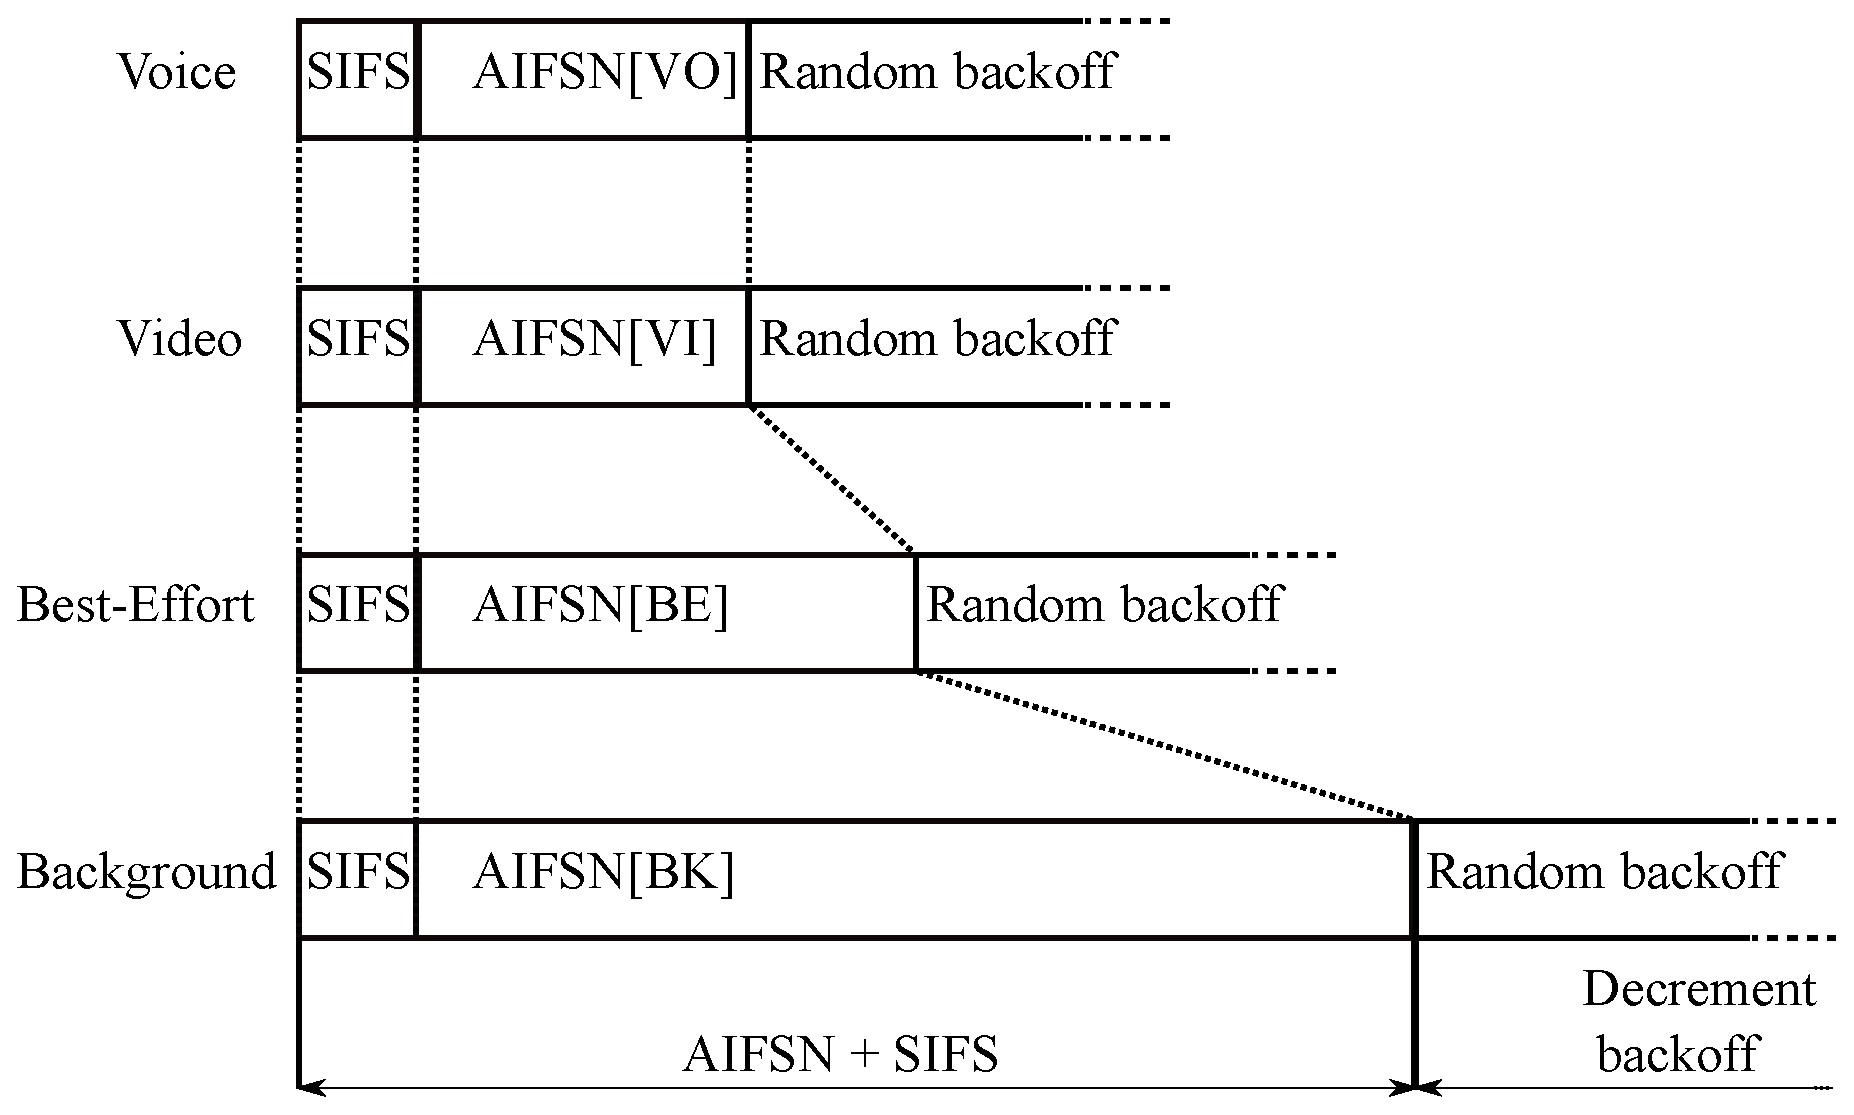
\includegraphics[width=\linewidth]{figures/AIFSN.eps}
		\caption{AIFSN values for each AC. From lowest (BK) to highest priority (VO).}
		\label{fig:AIFSN}
	\end{figure}

While being effective in providing traffic differentiation and priority, in principle EDCA is unable to eliminate collisions. For instance, two ACs from different contenders may draw the same random backoff and consequently attempt transmission in the same time slot, causing a collision. Collisions force a retransmission of the frame by repeating a contention after doubling the current CW. Furthermore, if two or more ACs within a node experience a backoff expiration at the same instant, a Virtual Collision (VC) will occur. VC are resolved by granting the channel to the highest priority AC, while doubling the CW for the lower priority ACs; just as it is done in the event of a real collision.

It follows directly from above that collisions waste channel time and thus contribute to the throughput degradation in WLANs. Moreover, the probability of collision increases as more contenders join the network, each one having four ACs attempting to gain access to the channel.

\subsection{Other contributions}
Because ACs in EDCA perform contention independently of the others, each AC mimics a station. This explains why the collision probability in EDCA is higher than in single-AC DCF networks with the same number of nodes. Furthermore, the contention parameters in EDCA work better in scenarios with low number of contenders, but often cause starvation of low priority ACs in crowded scenarios (see~\cite{990806} and Section~\ref{sim:results}).

Therefore, great efforts have been directed towards parameter adjustments in EDCA~\cite{throughputGuarantees,6614899,4594854}. For example, by dynamically adjusting the AIFS for each AC it is possible to maintain traffic differentiation while avoiding the starvation of low priority ACs. This is especially relevant in WLANs where all ACs are required to have effective throughput, like in~\cite{6614899}. Further, by randomising the AIFS values it is possible to increase the channel utilisation in EDCA~\cite{4594854}. Nevertheless, all these approaches either require information about the number of nodes participating in the contention, or inject additional traffic to the network, which may be unsuitable for crowded scenarios.

\section{Traffic Differentiation with CSMA/ECA}\label{section3}

\begin{figure*}[t!]
\centering
	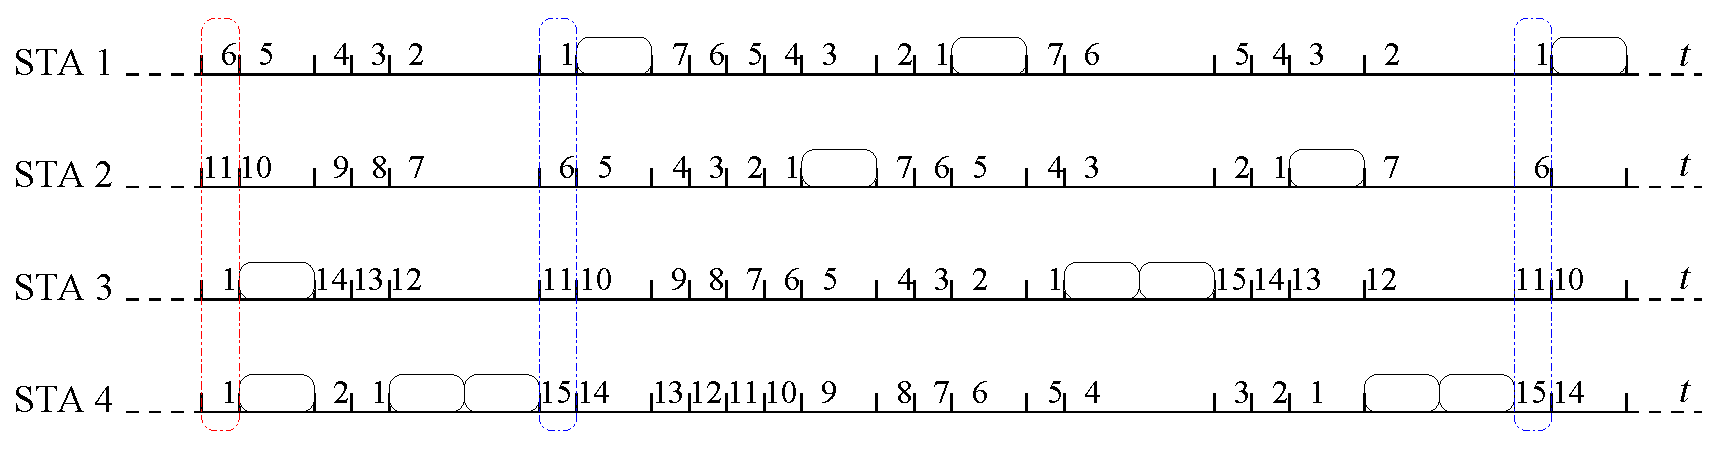
\includegraphics[width=0.8\linewidth]{figures/csma_eca_different_backoff_short.eps}
	\caption{An example of the temporal evolution of CSMA/ECA in saturation}
	\label{fig:ECA}
\end{figure*}
	
Carrier Sense Multiple Access with Enhanced Collision Avoidance~\cite{sanabria2014high, research2standards} is able to build collision-free schedules by using a deterministic backoff after successful transmissions. That is, if all saturated contenders are able to perform a successful transmission and then pick a deterministic backoff, they will not collide among each other in future transmissions.
	
When a packet arrives at an empty MAC queue, stations generate a random backoff $B\leftarrow\mathcal{U}[0,CW_{\min}-1]$, just as in DCF. Every passing empty slot decrements $B$ in one. When $B=0$, the station will attempt a transmission. If the transmission fails, the node will increment its backoff stage $k\in[0,m]$ in one (where $m$ is the maximum backoff stage of typical value $m=5$) and use another random backoff $B\leftarrow\mathcal{U}[0,CW(k)-1]$; where $CW(k)=2^{k}CW_{\min}$ is the contention window at backoff stage $k$. Otherwise, the successful station will then pick a deterministic backoff for its next transmission, $B_{\text{d}}\leftarrow \lceil CW_{\min}/2\rceil-1$. This value of $B_{\text{d}}$ is roughly equal to the expectation of a random backoff at the same backoff stage ($k=0$, in this case), making it fair and compatible with CSMA/CA stations~\cite{research2standards}.

\subsection{Supporting many more contenders with Hysteresis, Fair Share and the Schedule Reset mechanism}\label{scheduleReset}

CSMA/ECA is also capable of allocating many contenders in a collision-free schedule by not reseting the backoff stage $k$ after a successful transmission, as opposed to CSMA/CA. That is, a node at backoff stage $k$ would select $B_{\text{d}}\leftarrow \lceil CW(k)/2\rceil-1$ as its deterministic backoff after a successful transmission. This extension to CSMA/ECA is called Hysteresis. 

Hysteresis forces some contenders to have larger schedules than others, resulting in an unfair distribution of the network resources. This effect can be compensated by allowing nodes at backoff stage $k$ to transmit $2^{k}$ packets upon each transmission attempt. We call this extension Fair Share and it ensures an even distribution of the available throughput among contenders.

Figure~\ref{fig:ECA} shows a temporal example of CSMA/ECA with its extensions, namely, Hysteresis and Fair Share~\cite{sanabria2014high}. The \emph{STA-\#} labels denote the saturated contenders. The horizontal lines represent time, where the numbers are the number of empty slots left until the expiration of the backoff counter. In the figure, the first outline indicates a collision which forces STA-3 and STA-4 to increase their backoff stages ($k \leftarrow \min(k+1,m)$) and use a random backoff, $B\leftarrow\mathcal{U}[0,CW(k)-1]$. When STA-4's backoff expires, it will then transmit $2^{k}$ packets. Because the transmission was successful it uses $B_{\text{d}}=\lceil CW(k)/2\rceil-1$ as its deterministic backoff for the next transmission. Notice that once all stations transmit successfully collisions are eliminated.

CSMA/ECA with Hysteresis and Fair Share (CSMA/ECA$_{\text{Hys+FS}}$) is able to outperform CSMA/CA, as shown in the simulation results presented in Figures~\ref{fig:CAvsECA} and~\ref{fig:col-CAvsECA}. For the sake of clarity, Algorithm~\ref{alg:DCF} and Algorithm~\ref{alg:ECA} exemplify CSMA/CA and CSMA/ECA$_{\text{Hys+FS}}$ respectively.


	\begin{algorithm}[t]
	\While{the device is on}
	{
	  %\tcc{Initialize retransmission attempts.}
	  $r \leftarrow 0$; $k \leftarrow 0$\;
	  %\tcc{Initialize backoff counter.}
	  $B \leftarrow \mathcal{U}[0,2^k{\rm{CW}_{min}}-1]$\;
	  \While{there is a packet to transmit}{
	    %\tcc{Initialize $a$.}
	    \Repeat{($r = R$) or (success)}{
	      %\tcc{First, backoff.}
	      \While{$B>0$}{
	        wait 1 slot\;
	        $B \leftarrow B-1$\;
	      }
	      \colorbox{yellow}{Attempt transmission of 1 packet;}\\
	      \If{collision}{\label{collision}
	        %\tcc{Random backoff.}
	        $r \leftarrow r+1$\;
	        $k \leftarrow \min (k+1,m)$\;
	        $B \leftarrow \mathcal{U}[0, 2^k {\rm{CW}_{min}} -1]$\;\label{finalCollision}
	      }
	    }
	    $r \leftarrow 0$\;
	    \colorbox{yellow}{$k \leftarrow 0$;}\\
		 \eIf{success}{
	      %\tcc{Random backoff.}
	      \colorbox{yellow}{$B \leftarrow \mathcal{U}[0,2^{k}{\rm{CW}_{min}}-1]$;}\\\label{randomBackoff}
	    }
	    {
	      Discard packet\;
	      $B \leftarrow \mathcal{U}[0,2^k {\rm{CW}_{min}}-1]$\;
	    }
	  }
	  Wait until there is a packet to transmit\;
	}
	\caption{\small{CSMA/CA. $r$ indicates the number of retransmission attempts, while $R$ is the maximum retransmission attempts limit. When it is reached, the packet waiting for transmission is dropped.}}
	\label{alg:DCF}
	\end{algorithm}

	\begin{algorithm}[t]
	\While{the device is on}
	{
	  $r \leftarrow 0$ ; $k \leftarrow 0$ ; $k_{c} \leftarrow k$\;
	  $b \leftarrow \mathcal{U}[0,2^k\rm{CW}_{min}-1]$\;
	  \While{there is a packet to transmit}{
	    %\tcc{Initialize $a$.}
	    \Repeat{($r = R$) or (success)}{
	      %\tcc{First, backoff.}
	      \While{$B>0$}{
	        wait 1 slot\;
	        $B \leftarrow B-1$\;
	      }
	      \colorbox{yellow}{Attempt transmission of $2^k$ packets;}\\
	      \If{collision}{
	        %\tcc{Random backoff.}
	        $r \leftarrow r+1$\;
	        $k \leftarrow \min (k+1,m)$\;
	        $B \leftarrow \mathcal{U}[0, 2^k  \rm{CW}_{min} -1]$\;
	      }
	    }
	    $r \leftarrow 0$\;
	    %$s \leftarrow 0$\;
	    \eIf{success}{
	      %\tcc{Random backoff.}
	      \colorbox{yellow}{$B_{d} \leftarrow \lceil 2^{k}\rm{CW}_{min}/2\rceil-1$;}\label{deterministicBackoff}\\
		$B \leftarrow B_{d}$\;
	    }
	    {
	      Discard $2^{k_{c}}$ packets\label{discard}\;
%	      $k \leftarrow 0$\;
	      $B \leftarrow \mathcal{U}[0, 2^k \rm{CW}_{min}-1]$\;
	    }
	
	$k_{c} \leftarrow k$\;
	  }
	  Wait until there is a packet to transmit\;
	}	
	\vspace{0.2cm}
	\caption{CSMA/ECA$_{\text{Hys+FS}}$: $k_{c}$ refers to the contention backoff stage, that is, the backoff stage with which a contention for transmission is started. After $R$ retransmission attempts, Fair Share instructs the node to drop $2^{k_{c}}$ packets}
	\label{alg:ECA}
	\end{algorithm}
	
The main difference between Algorithm~\ref{alg:DCF} and Algorithm~\ref{alg:ECA}, and therefore between CSMA/CA and CSMA/ECA$_{\text{Hys+FS}}$ is that the latter uses a deterministic backoff after a successful transmission. This difference is highlighted at line~\ref{randomBackoff} and line~\ref{deterministicBackoff} of Algorithms~\ref{alg:DCF} and~\ref{alg:ECA}, respectively.

CSMA/ECA$_{\text{Hys+FS}}$ instructs nodes not to reset their backoff stage after a successful transmission. This is done in order to increase the cycle length and provide a collision-free schedule for many contenders, which is desirable in dense scenarios.

%The increment of the backoff stage and consequently the enlargement of the deterministic backoff are the result of previous collisions. In WLANs, collisions are assumed when the transmitter does not receive an Acknowledgement (ACK) packet from the receiver after a SIFS period following the transmission of the data frame. This means that channel imperfections preventing the reception of ACKs would be assumed as collisions by the senders, therefore, will also provoke an increase on the deterministic backoff in CSMA/ECA$_{\text{Hys+FS}}$.

Having a big deterministic backoff increases the time between successful transmissions. Furthermore, if not operating in a scenario with many nodes the empty slots between transmissions are not longer negligible and degrade the overall throughput of the system. For instance, if nodes withdraw from the contention their previously used slots will now be empty. Contenders should be aware of this issue and pursue opportunities to reduce their deterministic backoff without sacrificing too much in collisions. 

	\begin{figure}[t!]
	\centering
		\includegraphics[width=0.7\linewidth, angle=-90]{figures/throughput-perfectChannel.eps}
		\caption{Average aggregate throughput ($CW_{\min}=32$)\cite{sanabria2014high}}
		\label{fig:CAvsECA}
	\end{figure}
	
	\begin{figure}[t!]
	\centering
		\includegraphics[width=0.7\linewidth, angle=-90]{figures/collisions-perfectChannel.eps}
		\caption{Average aggregate number of collision slots ($CW_{\min}=32$)\cite{sanabria2014high}}
		\label{fig:col-CAvsECA}
	\end{figure}


The \emph{Schedule Reset} mechanism for CSMA/ECA$_{\text{Hys+FS}}$ introduced in~\cite{sanabria2014high} consists on finding the smallest collision-free schedule between a contender's transmissions and then change the node's deterministic backoff to fit in that schedule. Take a contender with a $B_{\text{d}}=31$ as an example. By listening to the slots between its transmissions, we are able to determine the availability of smaller (and possibly) collision-free schedules. 

Figure~\ref{fig:scheduleReset1} shows the slots between the transmissions of a contender with $B_{\text{d}}=31$. Starting from the left, the current $B_{\text{d}}=0$ means that the slot will be filled with the contender's own transmission. Each following slot containing either a transmission or a collision is identified with the number one, while empty slots are marked with a zero. Notice that the highlighted empty slots appear every eight slots, suggesting that a schedule reduction from $B_{\text{d}}=31$ to $B_{\text{d}}^{*}=7$ is possible. The schedule change is performed after the contender's next successful transmission. 

%coupled with an increase by one in the node's \emph{stickiness}~\cite{L_MAC2}. 

%\footnote{Trailing waiting periods, like the SIFS, are composed of empty slots. These allow nodes to decrement their backoff counters even after a collision or successful slots. Without loss of generality, the stations in our examples and simulations decrement their respective backoff counters by one after these kind of slots (see example in Figures~\ref{fig:ECA} and~\ref{fig:ecaQoS}).}

	\begin{figure}[t!]
	\centering
		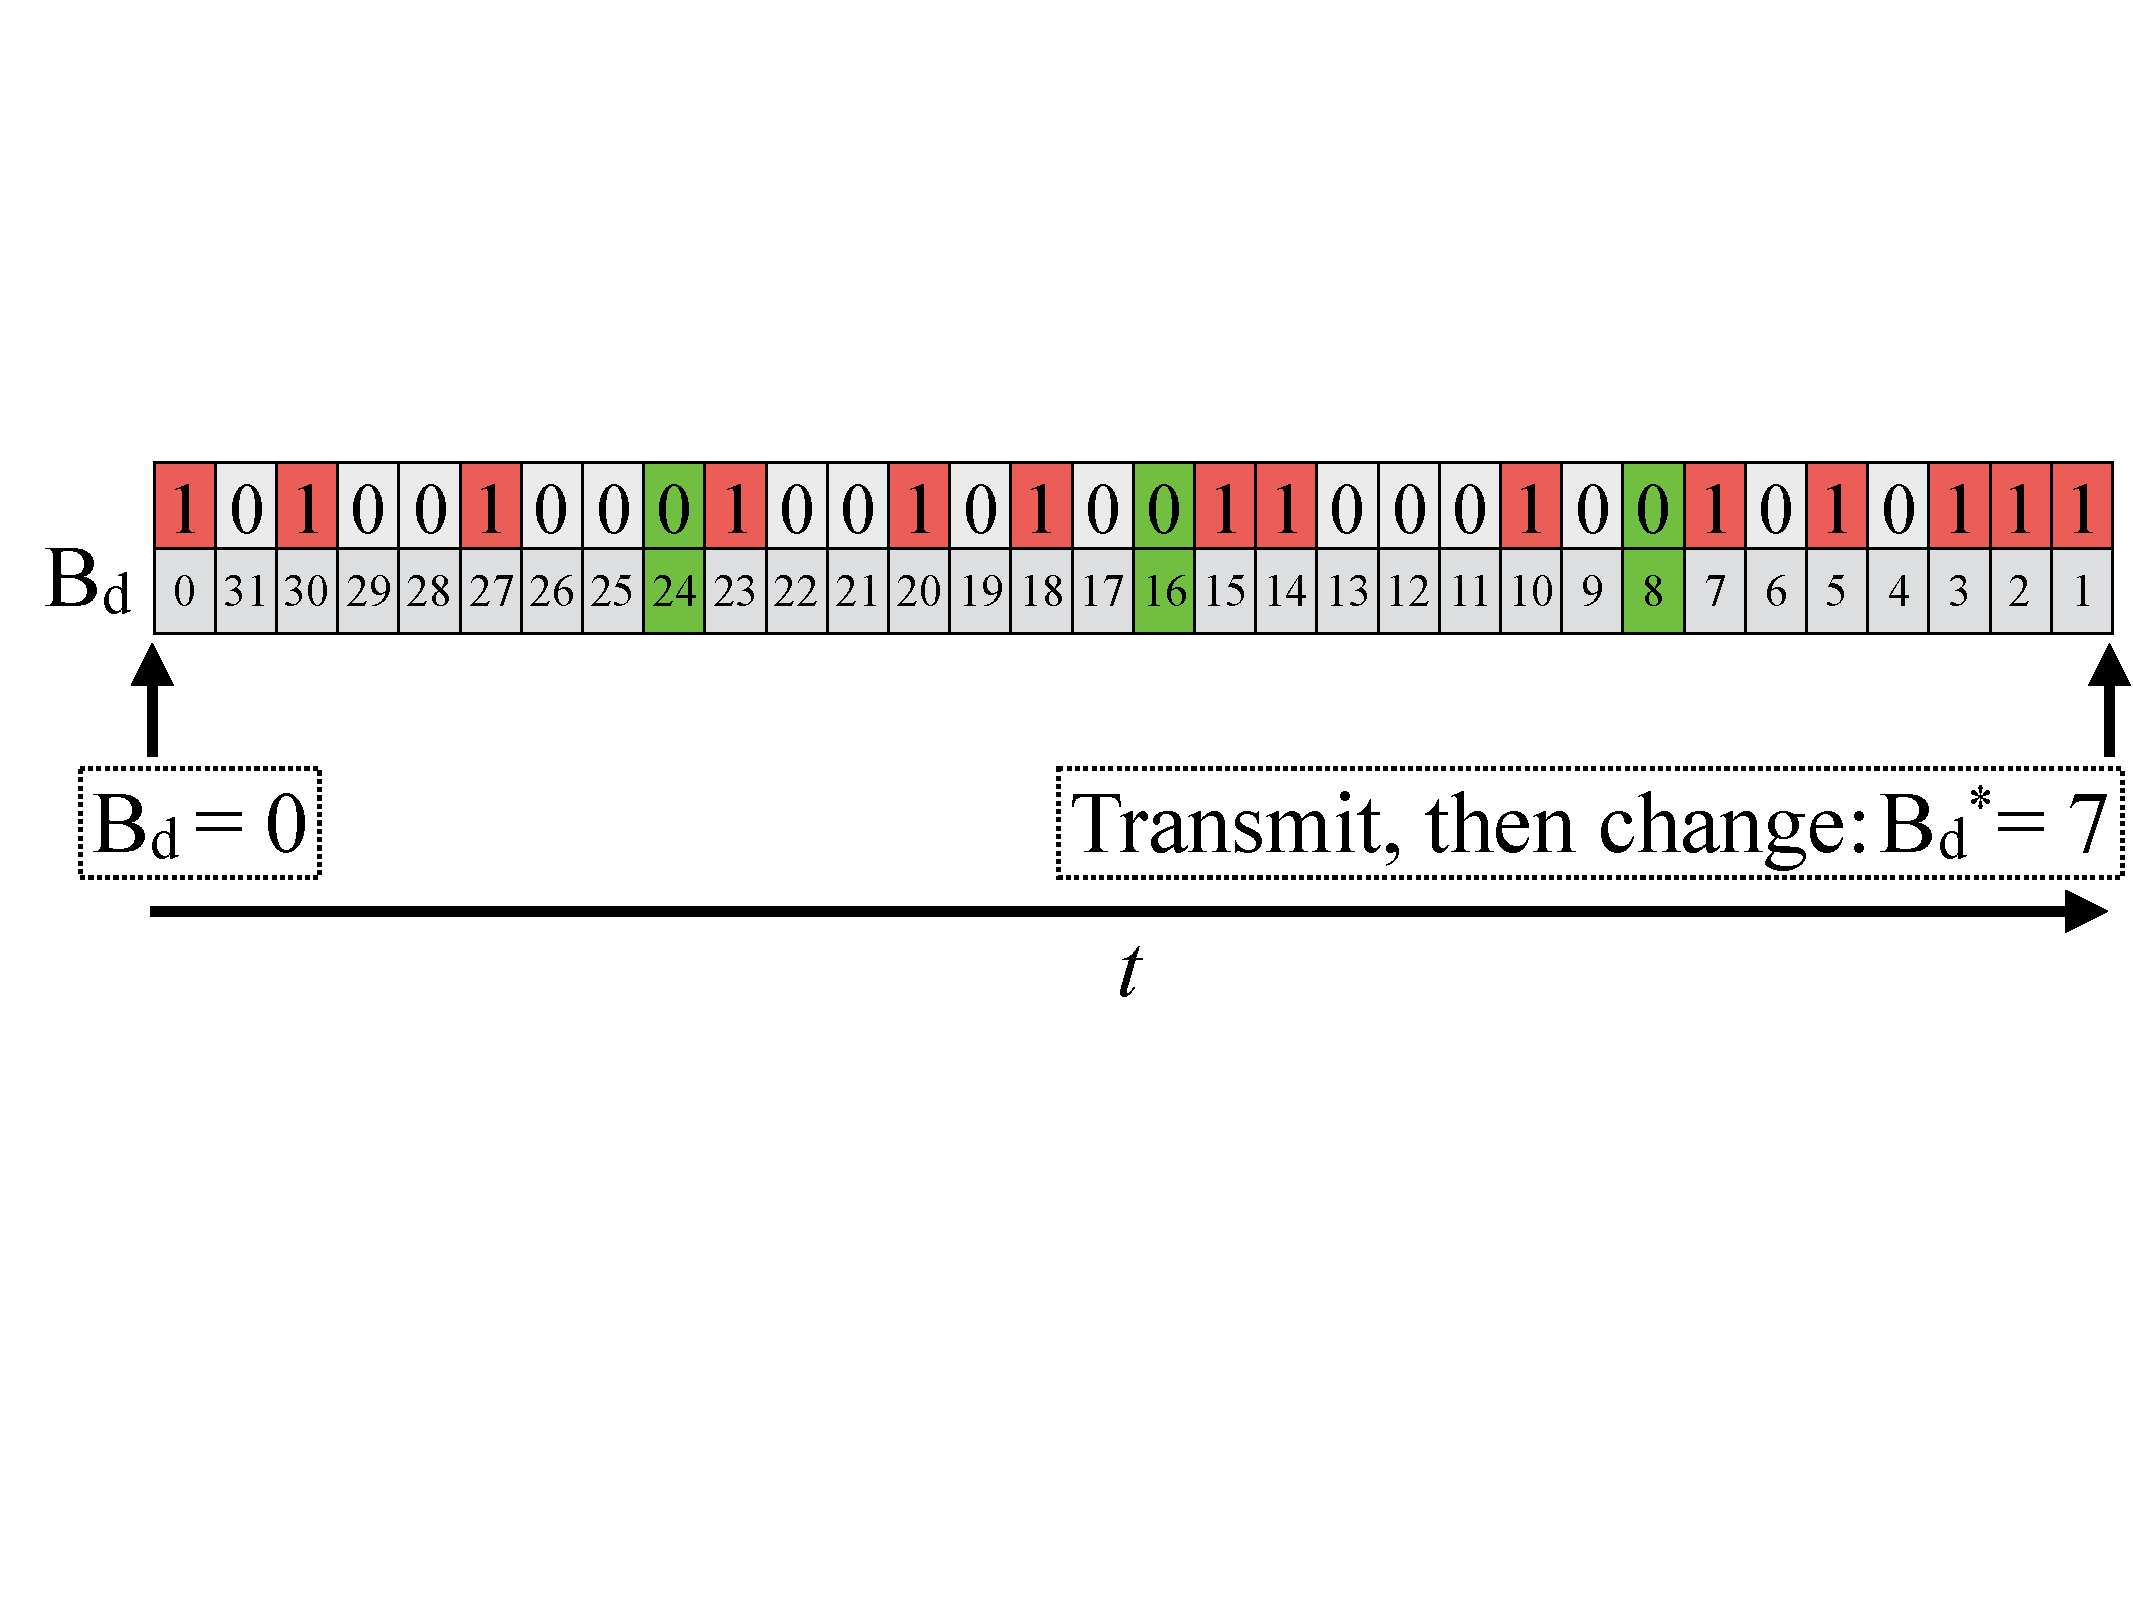
\includegraphics[width=\linewidth]{figures/scheduleReset.pdf}
		\caption{Example of the Schedule Reset mechanism (extracted from~\cite{sanabria2014high})}
		\label{fig:scheduleReset1}
	\end{figure}

Schedule Reset (SR) is implemented in CSMA/ECA$_{\text{Hys+FS}}$ by filling a bitmap $b$ of size $B_{\text{d}}+1$. Each bit $t,~t\in\{0,\ldots ,B_{\text{d}}\}$ in the bitmap is the result of a bitwise OR operation between its current value, $b[t]$ and the state of the slot; which equals to one when busy or zero when idle. After $\gamma$ consecutive successful transmissions (sxTx), the bitmap is evaluated. If a change of schedule is possible, it is executed just after the next successful transmission.

It is possible to configure Schedule Reset in two modes, namely \emph{conservative} and \emph{aggressive}. These modes relate to the number of consecutive transmissions needed to evaluate the bitmap, that is, $\gamma$. A conservative SR contains the information of all users' transmissions, therefore no additional collisions are introduced as a consequence of the schedule change. This implies a value of $\gamma=2^{m-1}CW_{\min}/B_{\text{d}}$. On the other hand, setting $\gamma=1$ triggers a bitmap evaluation after just two consecutive transmissions, rendering this choice of $\gamma$ the aggressive mode.

\begin{figure}[tb]
	\centering
		\includegraphics[width=0.7\linewidth, angle=-90]{figures/stickEv-throughput-overallOnly.eps}
		\caption{Average throughput and collisions with different levels of stickiness for CSMA/ECA$_{\text{QoS}}$ in non-saturation conditions (as explained in Section~\ref{subsect:simParams})}
		\label{fig:stickEv-throughput-overallOnly}
	\end{figure}

Aggressive Schedule Reset coupled with an increase in the Stickiness after an effective schedule change has proven to be suitable for noisy scenarios~\cite{sanabria2014high}, and the one used to provide the simulation results in Section~\ref{section4}. Stickiness is not a new concept to CSMA/ECA~\cite{barcelo2011tcf}. It simply instructs the contender to \emph{stick} to the deterministic backoff even in the event of \emph{stickiness} number of failed transmissions. This allows for a faster convergence towards a collision-free schedule. CSMA/ECA$_{\text{QoS}}$ with a default level of stickiness equal to $2$ has proven to provide the better combination of high throughput and low collisions, as shown in Figure~\ref{fig:stickEv-throughput-overallOnly}. Simulations results presented in Section~\ref{section4} imply an increase from ${\texttt{stickiness}}=2$ to ${\texttt{stickiness}}=3$ after a successful Schedule Reset.

%The Schedule Reset mechanism is activated after a complete schedule with a deterministic backoff, that is, the contender has performed $B_{d}/C$ successful transmissions, where $C$ is the number of slots in a complete schedule (like the exemplified in Section~\ref{ECAqosCollisionFree}).

\subsection{Incorporating multiple ACs into CSMA/ECA}
As shown before, CSMA/ECA and its extensions (referred to as CSMA/ECA$_{\text{Hys+FS}}$ from this point forward) are able to construct a collision-free schedule under saturated conditions, outperforming CSMA/CA. Furthermore, CSMA/ECA$_{\text{Hys+FS}}$ uses the same default contention parameters used by CSMA/CA, so the compatibility is maintained~\cite{sanabria2014high}.

Providing priority is to ensure a more frequent access to some ACs over others. In CSMA/ECA$_{\text{Hys+FS}}$ this is only subject to the deterministic backoff. That is, an AC using a shorter $B_{\text{d}}$ would in turn access the channel more often than those using a larger one. To maintain compatibility with EDCA, CSMA/ECA$_{\text{Hys+FS}}$ considers the same four ACs and CW values shown in Table~\ref{tab:EDCAparams}. 

Nevertheless, AIFS and TXOP are not fit for multiple CSMA/ECA$_{\text{Hys+FS}}$ queues. For instance, AIFS values are not required since differentiation is only provided by the deterministic backoff. The incorporation of different AIFS for each category would trigger Virtual Collisions that in turn may disrupt an existent collision-free schedule. Figure~\ref{fig:AIFSinECA} shows a VC in CSMA/ECA$_{\text{Hys+FS}}$ (indicated by the outline) consequence of using AIFS during a collision-free schedule.

	\begin{figure}[tb]
	\centering
		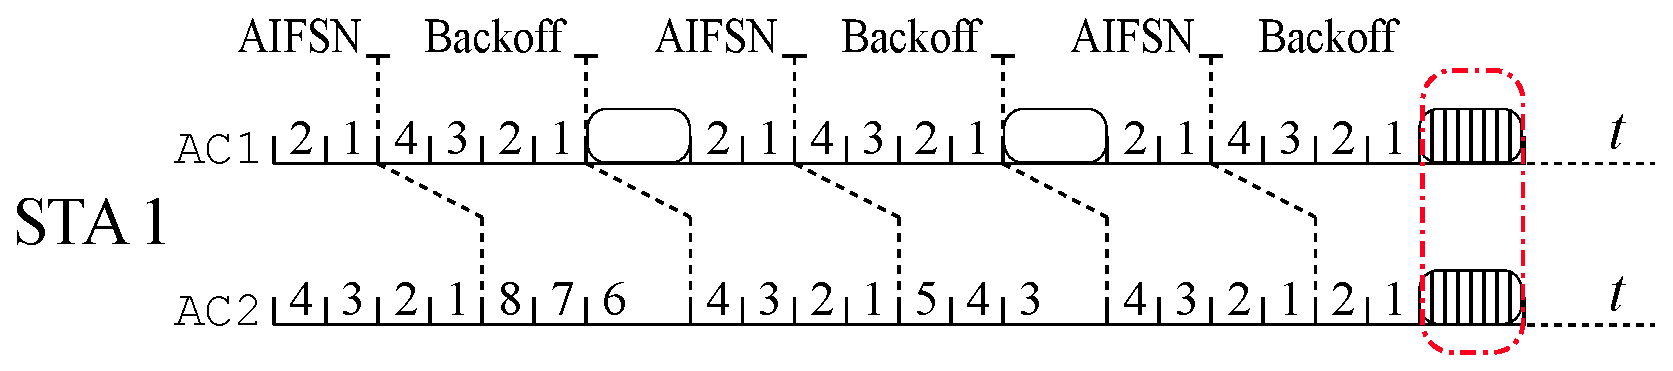
\includegraphics[width=\linewidth]{figures/AIFSwithECA.eps}
		\caption{Example temporal evolution of CSMA/ECA$_{\text{Hys+FS}}$ with two ACs using AIFS resulting in a virtual collision. Only considering AIFSN values of 2 and 4, $B_{\text{d}}$ of 4 and 8 for AC1 and AC2 respectively}
		\label{fig:AIFSinECA}
	\end{figure}


TXOP in EDCA ensures that all traffic from the same category receives on average the same channel time rather than the same throughput. In contrast, CSMA/ECA$_{\text{Hys+FS}}$'s goal through Fair Share is to provide close to equal average throughput to same-priority ACs. We leave the elaboration of an adaptive Fair Share which ensures resource fairness rather than throughput fairness as a future research topic.
%Nevertheless, this can be misleading. Take two low same-priority ACs, if using different transmission rates it will take different periods of time to complete each transmission. This defies the purpose of TXOP given that the network resources are not evenly shared. 

As EDCA extends DCF into four ACs, similarly there is an instance of CSMA/ECA$_{\text{Hys+FS}}$ for each AC. We will refer to CSMA/ECA$_{\text{Hys+FS}}$ with multiple ACs as CSMA/ECA$_{\text{QoS}}$ from here forward. Table~\ref{tab:ecaQosParams} shows the CW as well as the lowest and largest $B_{\text{d}}$ for ACs in CSMA/ECA$_{\text{QoS}}$.

Figure~\ref{fig:ecaQoS} shows an example of CSMA/ECA$_{\text{QoS}}$ with two contenders and two ACs; where AC1 has higher priority than AC2. In the figure, the first outline indicates a VC between AC1 and AC2 from STA-2. VC in CSMA/ECA$_{\text{QoS}}$ are handled just as in EDCA, that is, the AC with the highest priority is granted access to the channel, while the other ACs involved in the VC double their contention windows and use a random backoff for the next transmission. Consequently, AC1 from STA-2 successfully transmits and then uses $B_{\text{d}}=\frac{2^{0}CW_{\min}[\text{AC1}]}{2}-1= 3$.

Still on Figure~\ref{fig:ecaQoS}, the second outline indicates a collision between STA-2's AC2 and AC1 from STA-1. At this moment in time STA-2 AC2's backoff stage has been increased in two occasions ($k[\text{AC2}]=2$). When said AC2 is able to transmit, it sends $2^{k[\text{AC2}]}$ packets according to Fair Share. Then, it uses a deterministic backoff, $B_{\text{d}}=\frac{2^{k[\text{AC2}]}CW_{\min}[\text{AC2}]}{2}-1=31$.

	\begin{figure*}[tb]
	\centering
		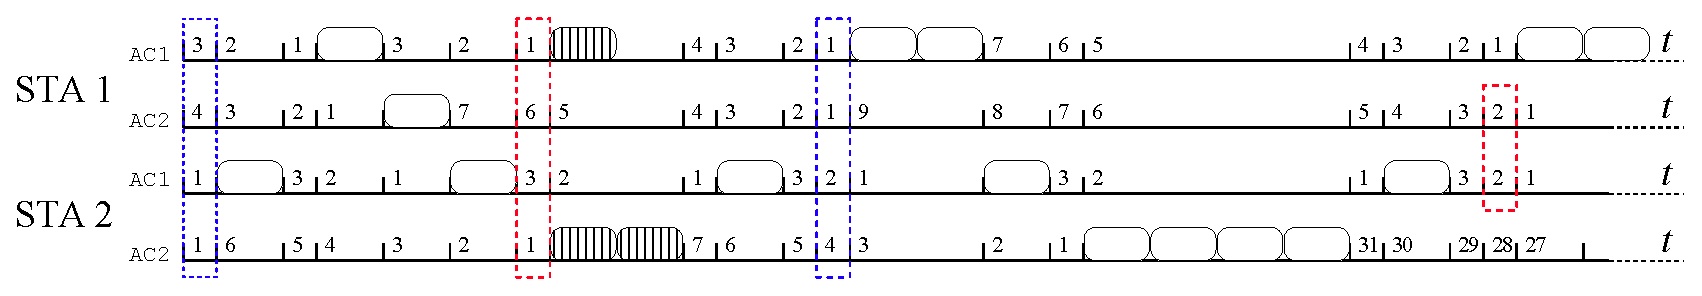
\includegraphics[width=0.9\linewidth]{figures/csma-eca-hew-oldScheme-fixed.eps}
		\caption{An example of the temporal evolution of CSMA/ECA$_{\text{QoS}}$ in saturation ($CW_{\min}[\text{AC1,AC2}]=[8,16]$; $m[\text{AC1,AC2}]=[5,5]$)}
		\label{fig:ecaQoS}
	\end{figure*}

The third outline in Figure~\ref{fig:ecaQoS} indicates an VC in STA-1, which is resolved allowing AC1 and deferring AC2's transmission using a random backoff with a doubled CW. A future collision between STA-2's AC1 and AC2 from STA-1 is highlighted by the last outline.

\subsection{Collisions and Virtual Collisions-free operation using Smart Backoff}\label{ECAqosCollisionFree}
Consider a complete schedule of length $C=2^{m}CW_{\min}$, and $m=5$. With CSMA/ECA$_{\text{Hys+FS}}$ and a single AC it is possible to allocate a collision-free transmission slot for up to $C/2=512$ contenders (the highest $B_{\text{d}}+1$ for AC Legacy in Table~\ref{tab:ecaQosParams}). Nevertheless, with CSMA/ECA$_{\text{QoS}}$ and all ACs in saturation each contender mimics the behaviour of four saturated nodes (one for each AC). This means that the total number of supported collision-free contenders will be reduced in order to provide a transmission slot for all the ACs in the network. If all the ACs are in saturation, i.e., have a packet to transmit, CSMA/ECA$_{\text{QoS}}$ can provide collision-free operation for up to $2^{m[\text{VO}]}CW_{\min}[\text{VO}]/2=8$ contenders, where $m[\text{VO}]$ is the maximum backoff stage of the AC with the smallest $CW_{\max}$. Even-though Table~\ref{tab:ecaQosParams} provides CSMA/ECA$_{\text{QoS}}$'s default contention parameters, these will be adjusted in Section~\ref{sim:results} in order to support more contenders while in saturation.

VCs in CSMA/ECA$_{\text{QoS}}$ force lower priority ACs to defer their transmissions using a random backoff. Therefore, VCs can disrupt any existent collision-free schedule in CSMA/ECA$_{\text{QoS}}$, wasting channel time recovering from collisions and degrading the overall throughput. Given that all AC's backoff counters are known to the contender, there is nothing preventing it from using this information to avoid future VCs.

CSMA/ECA$_{\text{QoS}}$ eliminates VCs by picking a $B[\text{AC}]$ that is not equal to any of the other AC's counters. This is exemplified in Figure~\ref{fig:smartBackoff1}. The figure shows a contender with four ACs and $B_{\text{d}}[4]=[4,8,16,16]$, for AC1 to AC4 respectively. AC1 effectively transmits, but AC3 suffers from a VC. It then selects a random backoff, $B[\text{AC3}]=24$, which is different from any other AC's counters but do not consider the deterministic backoff selected by successful ACs. To eliminate future VCs in CSMA/ECA$_{\text{QoS}}$ the successes of other ACs's transmissions should also be taken into account. This is achieved by selecting a number whose absolute difference with each of the other AC's counters is not a multiple of each comparison's smallest deterministic backoff. Algorithm~\ref{alg:smartBackoff} shows the process of selecting what is referred to as a \emph{Smart Backoff} in CSMA/ECA$_{\text{QoS}}$. It shows four ACs, although it can used to eliminate VCs with as many ACs as needed. Smart Backoff is used instead of a random backoff in CSMA/ECA$_{\text{QoS}}$.

%Nevertheless, because CSMA/ECA$_{\text{QoS}}$ ACs use a deterministic backoff after successful transmissions the selected $B[\text{AC3}]$ will eventually collide with AC1's next sixth successful transmission.

	\begin{algorithm}[t]
		$AC:=4$\tcp*[l]{number of Access Categories}
		$CW_{\min}[AC]$\tcp*[l]{$CW_{\min}$ for all ACs}
		$B_{\text{d}}[AC]$\tcp*[l]{$B_{\text{d}}$ for all ACs}
		$B[AC]$\tcp*[l]{current $B$ from all ACs}
		$k[AC]$\tcp*[l]{current backoff stage}
		$F[AC]:=\{0\}$\;
		$Cb[AC]:=\{0\}$\;
		\tcp{}\tcp{looking for a suitable $B[i]$; $i\in[1,AC]$}\tcp{}
		\While{$($F$~\neq 1)$ or $($Cb$~\neq 1)$}	
		{
			$B[i]\gets\mathcal{U}[0,2^{k[i]}{CW_{\min}[i]}]$\;
			\For{$(j = 1; j\leq \text{AC};j++)$}
			{
				\If{$(j\neq i)$}{
					$F[j]\gets |B[i]-B[j]|$~mod~$[\min(B_{\text{d}}[i],B_{\text{d}}[j])]$\;
					\If{$(F[j]\neq 0)$} 
					{	
						$F[j]\gets 1$\;
					}
					\eIf{$(B[i]\neq B[j])$}{
						$Cb[j]\gets 1$\;
					}{
						$Cb[j]\gets 0$\;
					}
				}
			}
			
			
		}
		\Return $(B[i])$\;
		\vspace{0.2cm}
		\caption{Smart Backoff: eliminating Virtual Collisions in CSMA/ECA$_{\text{QoS}}$}
		\label{alg:smartBackoff}
	\end{algorithm}

What results from Algorithm~\ref{alg:smartBackoff} is a Smart Backoff counter that will not cause a VC on the next transmission attempts.

	\begin{table}[tb]
		\centering
		\caption{Deafult CSMA/ECA$_{\text{QoS}}$ contention parameters}
		\label{tab:ecaQosParams}
		\begin{tabular}{|c|c|c|c|c|c|}
			\hline
			{\bfseries AC} & {\bfseries CW$_{\min}$} & {\bfseries CW$_{\max}$} & {\bfseries m} & {\bfseries lowest $B_{\text{d}}$} & {\bfseries highest $B_{\text{d}}$}\\
			\hline
			BK		       &	32				&		1024		  & 		5	&			15		        &		511\\
			BE		       &	32				&		1024		  &		5	&			15		        &		511\\
			VI		       &	16				&		32			  & 		1	&			7		        &		15\\
			VO		       &	8				&		16		 	 & 		1	&			3		        &		7\\
			Legacy	       &	32				&		1024		  & 		5	&			15		        &		511\\
			\hline
		\end{tabular}
	\end{table}

	\begin{figure}[tb]
	\centering
		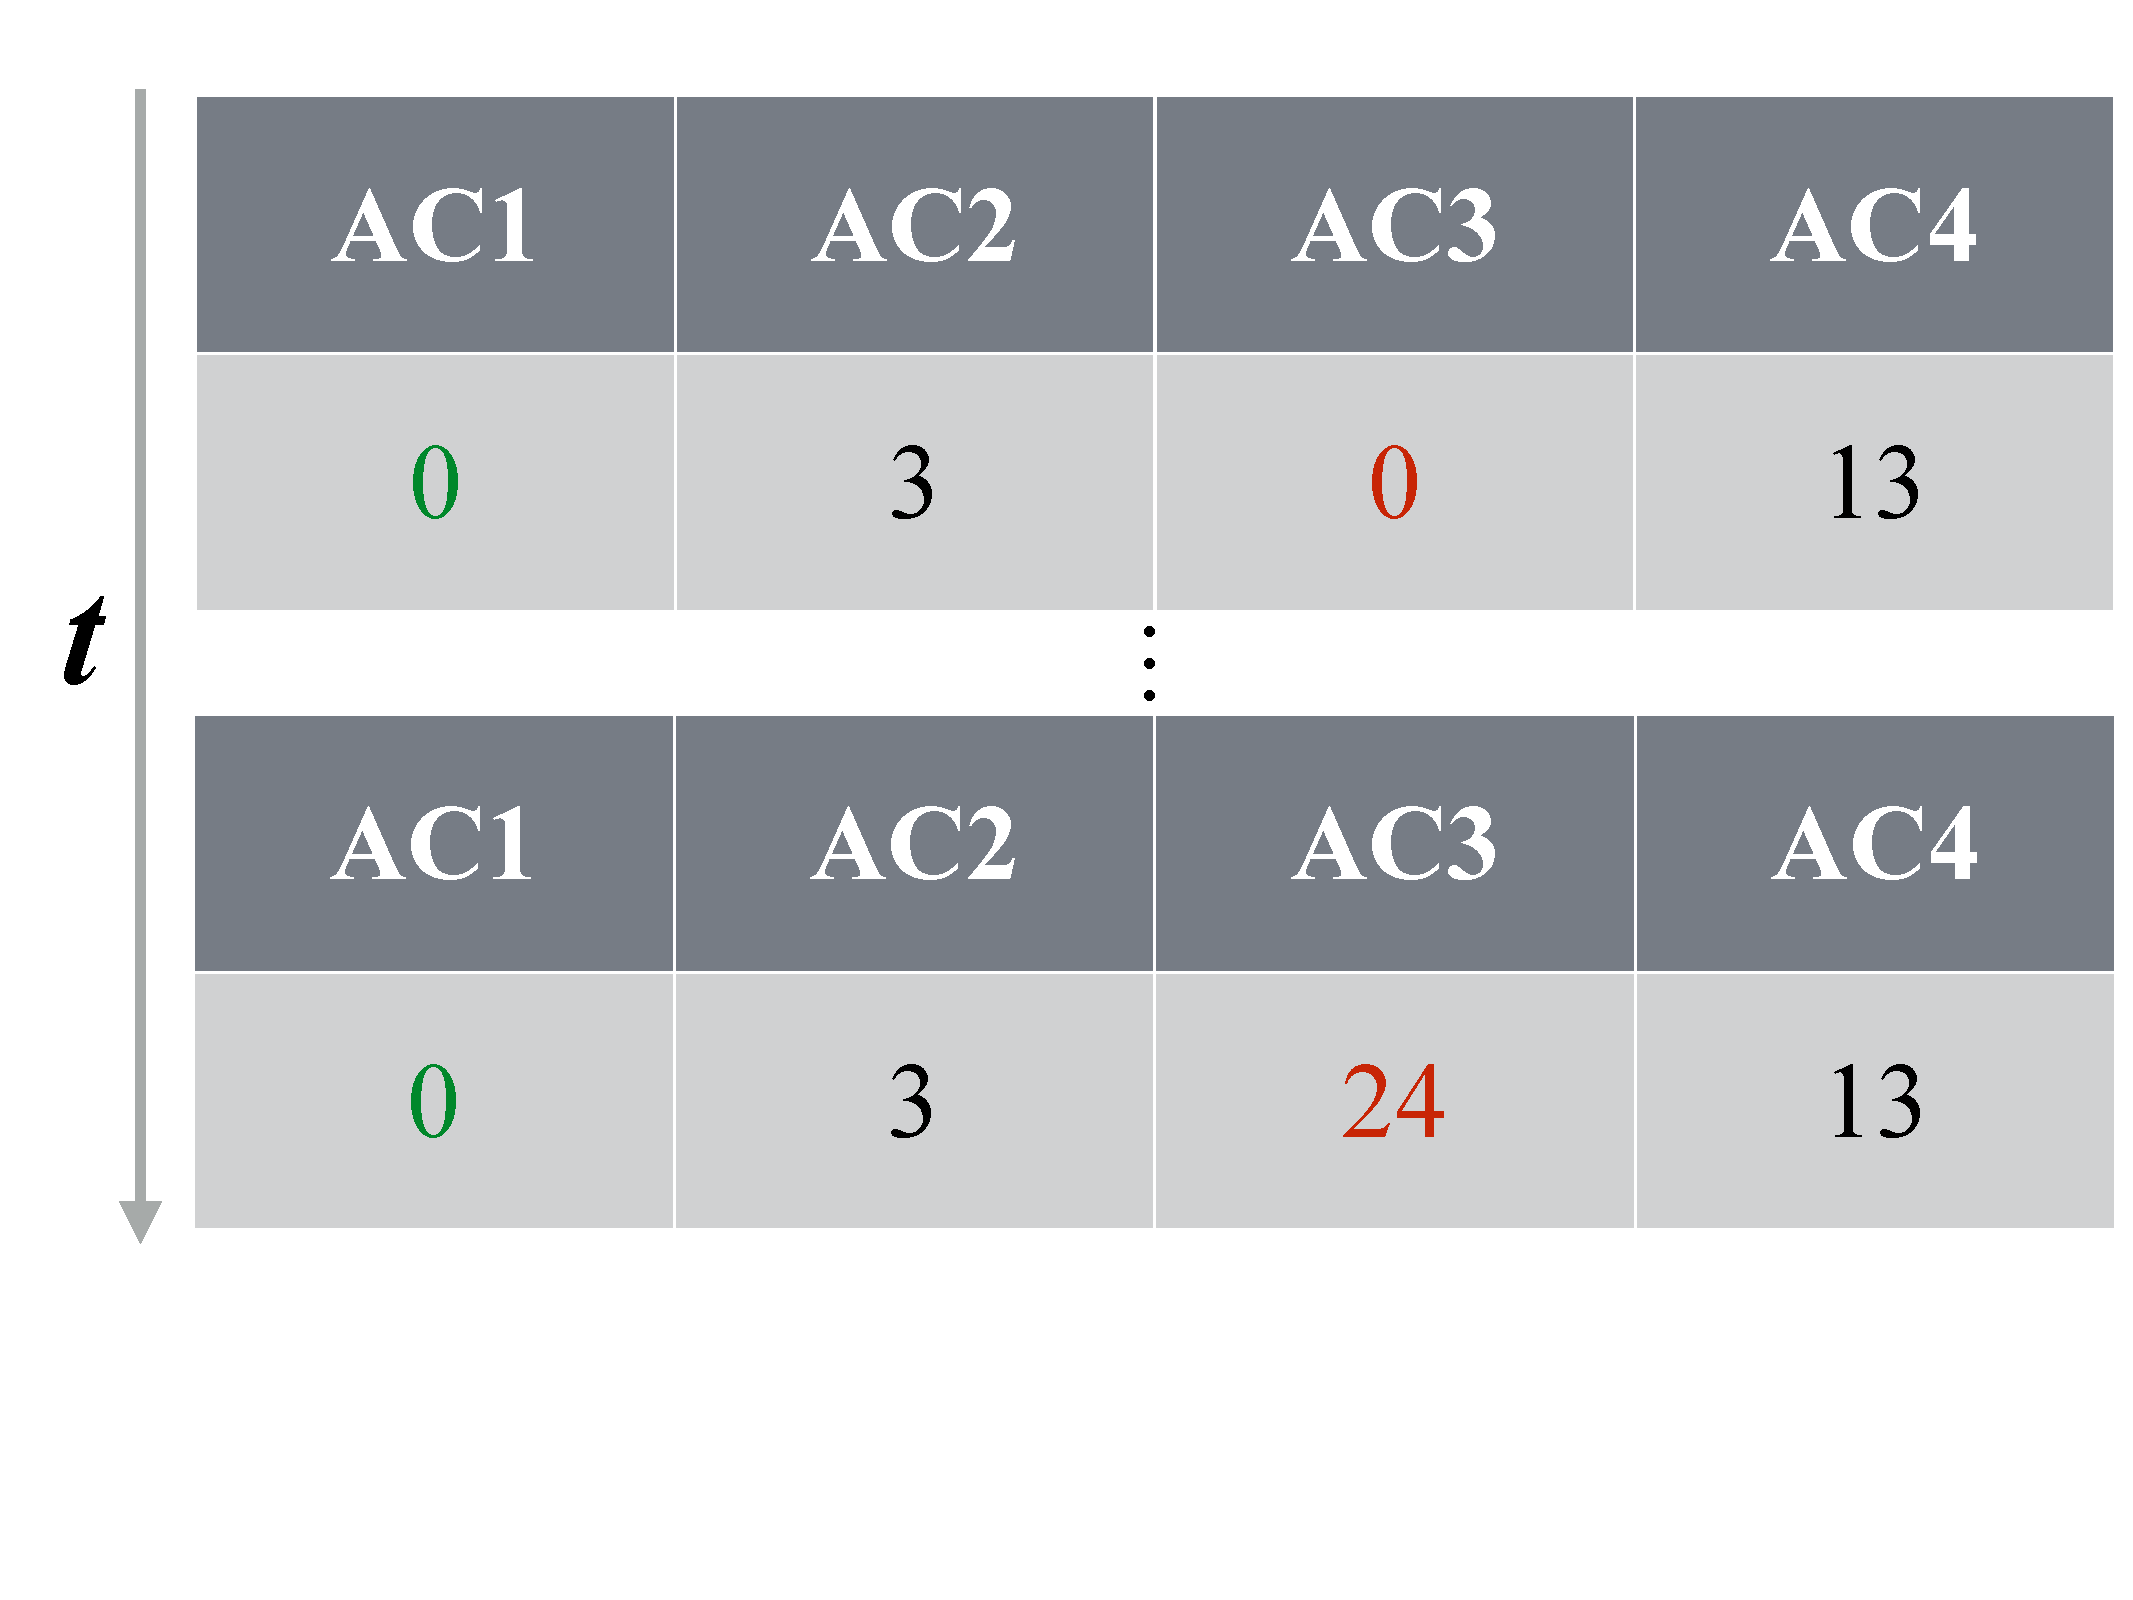
\includegraphics[width=0.8\linewidth]{figures/smartBackoff1.pdf}
		\caption{Four AC backoff counters in a CSMA/ECA$_{\text{QoS}}$ node with $B_{\text{d}}[4]=[4,8,16,16]$. After a VC or collision, the new random backoff counter must not be equal to any other AC's counter}
		\label{fig:smartBackoff1}
	\end{figure}

\section{Performance Evaluation}\label{section4}
In order to test the traffic differentiation capabilities of CSMA/ECA$_{\text{QoS}}$ we have used a customised version of the COST simulator~\cite{COST}, which is available via~\cite{CSMA-ECA-HEW}. If not expressed otherwise, each point in the presented figures (including Figures~\ref{fig:CAvsECA} and \ref{fig:col-CAvsECA}) is obtained from averaging fifty executions of duration equal to one hundred seconds. Further considerations:
	\begin{itemize}
		\item Unspecified parameters follow the IEEE 802.11n ($2.4$~GHz) standard.
		\item All nodes can be assumed to be in communication range with each other.
		\item Not using Request-to-Send (RTS) or Clear-to-Send (CTS) messages.
		\item Collisions are assumed to take as much channel time as successful transmissions.
	\end{itemize}

Additionally, Table~\ref{tab:mac-params} provides information about relevant PHY and MAC parameters used in the simulator.
	\begin{table}
		\centering
		\caption{PHY and MAC parameters for the simulations}
		\label{tab:mac-params}
		\begin{tabular}{|c|c|}
			\hline
			\multicolumn{2}{|c|}{{\bfseries PHY}}\\
			\hline
			{\bfseries Parameter} & {\bfseries Value}\\
			\hline
			PHY rate & 65~Mbps\\
			Empty slot & $9~\mu s$\\
			DIFS & $28~\mu s$\\
			SIFS & $10~\mu s$\\
			\hline
			\multicolumn{2}{|c|}{{\bfseries MAC}}\\
			\hline
			{\bfseries Parameter} & {\bfseries Value}\\
			\hline
			Maximum retransmission attempts & 7\\
			Packet size (Bytes) & 1024\\
			MAC queue size (Packets) & 1000\\
			\hline
		\end{tabular}
	\end{table}
	
	\begin{table}[t]
		\centering
		\caption{Updated CSMA/ECA$_{\text{QoS}}$ contention parameters for the simulations}
		\label{tab:newQoSparams}
		\begin{tabular}{|c|c|c|c|c|c|}
			\hline
			{\bfseries AC} & {\bfseries CW$_{\min}$} & {\bfseries CW$_{\max}$} & {\bfseries m} & {\bfseries lowest $B_{\text{d}}$} & {\bfseries highest $B_{\text{d}}$}\\
			\hline
			BK		       &	32				&		1024		  & 		5	&			15		        &		511\\
			BE		       &	32				&		1024		  &		5	&			15		        &		511\\
			VI		       &	16				&		512		  & 		5	&			7		        &		255\\
			VO		       &	8				&		256		  & 		5	&			3		        &		127\\
			Legacy	       &	32				&		1024		  & 		5	&			15		        &		511\\
			\hline
		\end{tabular}
	\end{table}
	
Apart from the assumptions presented above, the following provide details about the traffic source generator, channel conditions and overall scenarios to be evaluated. Then, simulation results for achieved throughput, number of collisions and time between successful transmissions are presented.

\subsection{Simulation parameters}\label{subsect:simParams}
\subsubsection{Traffic conditions}
There are two main scenarios regarding traffic generation in a node. The \emph{saturated} traffic condition refers to a node that always has a packet for transmission in its MAC queue. On the other hand, a \emph{non-saturated} node  can also empty its MAC queue and withdraw from the channel contention. These states do not fall far from reality, for instance, a node might be in saturation while it is performing a file transfer. But if instead the node is only uploading a short file, does nothing for a period of time and then continues to perform a voice call over the network, its traffic will be considered to be non-saturated over that period of time.

In our simulator we mimic this behaviour by defining a packet arrival rate ($\Delta\text{P}$). To simulate a saturated network, for instance, we set $\Delta\text{P}$ in every node to the channel capacity. If non-saturated traffic is the goal, $\Delta\text{P}$ will be set to a value way below the system maximum aggregated throughput in order to induce periods of inactivity upon each node. After extensive tests, $\Delta\text{P}=2\text{Mbps}$ has proved to provide satisfactory results.

The performance in non-saturation for EDCA and CSMA/ECA$_{\text{QoS}}$ will be greatly dependent on the share of $\Delta\text{P}$ each AC gets, that is, the percentage of generated traffic that is going to be assigned to each AC. These shares, denoted $\Delta\text{P}_{\text{AC}}$ are distributed in the following way: $\Delta\text{P}_{\text{BK}}=0.4\Delta\text{P}$, $\Delta\text{P}_{\text{BE}}=0.3\Delta\text{P}$, $\Delta\text{P}_{\text{VI}}=0.15\Delta\text{P}$ and $\Delta\text{P}_{\text{VO}}=0.15\Delta\text{P}$. These values comply with the desired scenario.

	
\subsubsection{Channel errors}
The inability to receive an ACK frame is handled as a collision, both in EDCA and CSMA/ECA$_{\text{QoS}}$. This could happen due to channel imperfections preventing the receiver from decoding the transmissions. In order to simulate the effects of channel errors over the MAC protocol, we define the likelihood of a packet not being acknowledged, $p_e$. It affects every packet independently. That is, for every packet being transmitted we draw a number from a random variable $X\sim\mathcal{U}[0,1]$, if the number drawn is lower than $p_e$ the packet will not be acknowledged. In the case of an aggregation of several packets, it is considered a failed transmission only if all packets in the aggregation are affected negatively by $p_e$. A value of $p_e=0.1$ has been selected for the simulations.

\subsubsection{Scenarios to test}
In this work we propose two main scenarios: saturation and non-saturation. The non-saturation scenario will be composed of nodes with $\Delta\text{P}=2\text{Mbps}$.

%////////////////////////////////////////////////////////////////////////////////////
%///////////////////////////////////////%Results%////////////////////////
%///////////////////////////////////////////////////////////////////////////////////

\begin{figure*}[tb]
	\centering
		\includegraphics[width=0.55\linewidth,angle = -90]{figures/multiplot-sat-perfect.eps}
		\caption{Average Aggregated Throughput and Collisions for a) EDCA, b) CSMA/ECA$_{\text{QoS}}$ and c) CSMA/ECA$_{\text{QoS}}$ with parameters from Table~\ref{tab:newQoSparams} in saturation}
		\label{fig:multiplotSat}
\end{figure*}

\begin{figure*}[tb]
	\centering
		\includegraphics[width=0.55\linewidth,angle = -90]{figures/multiplot-unsat-error-0-1.eps}
		\caption{Average Aggregated Throughput, Collisions and Time Between Successful Transmissions for a) EDCA and b) CSMA/ECA$_{\text{QoS}}$ and c) CSMA/ECA$_{\text{QoS}}$ network (without Fair Share) in non-saturation}
		\label{fig:multiplotUnsat}
\end{figure*}
	
\begin{figure*}[t]
	\centering
		\includegraphics[width=0.55\linewidth,angle = -90]{figures/multiplot-combined-unsat-error-0-1.eps}
		\caption{Average aggregated throughput, Collisions and time between successful transmissions for a) EDCA nodes and b) CSMA/ECA$_{\text{QoS}}$ nodes and c) CSMA/ECA$_{\text{QoS}}$ network (without Fair Share) nodes in a 50\%-50\% mixed non-saturated network}
		\label{fig:multiplotCombinedUnsat}
\end{figure*}

\subsection{Simulation Results}\label{sim:results}
\subsubsection{System throughput and collisions}
\begin{itemize}
\item\underline{Saturation:} Figure~\ref{fig:multiplotSat} gathers the simulation results for average aggregated throughput and collisions in a saturated network. Referring to EDCA results as Figure~\ref{fig:multiplotSat}-a,  it shows that the AC with the highest priority, AC[VO]\footnote{Starting at this point, ACs will be referred to as AC[\emph{x}], where `\emph{x}' is the abbreviation of the AC name, as in Table~\ref{tab:prioritiesMap}.}, achieves greater throughput than the others. This is a direct consequence of effective traffic differentiation in EDCA. The lower row of Figure~\ref{fig:multiplotSat} shows the total number of collisions as well as the average percentage of collisions suffered by each AC. 

Figure~\ref{fig:multiplotSat}-a also shows that AC[BK] is not able to achieve significant throughput for a high number of contenders. This is because its transmission attempts are being deferred in order to serve the high priority ACs. Furthermore, EDCA collisions show that at around 30 contenders AC[BE] also starts to get its transmission attempts deferred, easing the contention process for high priority ACs. This is the main reason of the overall throughput increase seen in Figure~\ref{fig:multiplotSat}-a at around 30 nodes.

Figure~\ref{fig:multiplotSat}-b shows the average aggregated throughput and collisions of a saturated CSMA/ECA$_{\text{QoS}}$ network using the default contention parameters (see Table~\ref{tab:ecaQosParams}). These settings do not allow the construction of collision-free schedules for many contenders. This is evidenced by the high number of collisions at around 20 contenders. Moreover, the figure shows CSMA/ECA$_{\text{QoS}}$ throughput decreasing faster than EDCA.

To allow the construction of collision-free schedules, the contention parameters for CSMA/ECA$_{\text{QoS}}$ are modified to the ones shown in Table~\ref{tab:newQoSparams}. These new parameters allow the construction of larger collision-free schedules, making it possible to achieve collision-free operation with a larger number of contenders. Figure~\ref{fig:multiplotSat}-c provides throughput and collisions results with these new contention parameters. The figure shows higher throughput for a wider number of contenders, as opposed to EDCA, where it decreases rapidly as contenders join the network. Further, collisions start to increase at around 32 contenders, which is the maximum number of saturated collision-free contenders supported with the updated contention parameters. It is relevant to highlight that unlike EDCA, CSMA/ECA$_{\text{QoS}}$ is able to accommodate transmissions for every AC when there is a high number of contenders (e.g.: $N\geq 40$). In the same manner, Figure~\ref{fig:multiplotSat}-c also shows a clear reduction in the number of collisions when using CSMA/ECA$_{\text{QoS}}$.

The updated parameters for CSMA/ECA$_{\text{QoS}}$ (Table~\ref{tab:newQoSparams}) make a tradeoff between throughput and aggressiveness. Even-though allowing CSMA/ECA$_{\text{QoS}}$'s deterministic backoffs to grow past EDCA's default parameters increases the time between successful transmissions (as shown in the following Figure~\ref{fig:multiplotUnsat}), it prevents the starvation of low priority ACs and provide a greater overall throughput (due to a reduction in the number of collisions and the aggregation performed by Fair Share).


\item\underline{Non-Saturation:}

In the non-saturation scenario nodes in the network have $\Delta\text{P}=2$Mbps. Moreover, the shares of $\Delta\text{P}$ assigned to each AC are defined in Section~\ref{subsect:simParams}. Results are derived from simulations performed with $p_e=0.1$.

	\begin{table}[t]
		\centering
		\caption{Saturation points in non-saturation scenarios ($N$)}
		\label{tab:satPoints}
		\begin{tabular}{|c|c|c|c|c|}
			\hline
			{\bfseries Protocol} 				& {\bfseries BK} & {\bfseries BE} & {\bfseries VI} & {\bfseries VO}\\
			\hline
			EDCA						&	10		&	16		&		22	&	22\\	
			\hline
			CSMA/ECA${\text{QoS}}$		&	14		&	16		&		36	&	50\\
			\hline
			CSMA/ECA${\text{QoS}}$ w/o FS	&	10		&	16		&		28	&	28\\
			\hline
		\end{tabular}
	\end{table}

Figure~\ref{fig:multiplotUnsat} shows the (from top to bottom row) average aggregated throughput, collisions and time between successful transmissions for (from left to right column) a) EDCA, b) CSMA/ECA$_{\text{QoS}}$ and c) CSMA/ECA$_{\text{QoS}}$ without Fair Share (both CSMA/ECA$_{\text{QoS}}$ results using the contention parameters presented in Table~\ref{tab:newQoSparams}). In Figure~\ref{fig:multiplotUnsat}-a, EDCA throughput keeps increasing up until one of its ACs reaches saturation due to starvation. This is the case of AC[BK] at around $N=10$. It is only at around $N=24$ where the rest of ACs get completely saturated. At this point, both the throughput and collision figures for EDCA start to resemble the ones presented in the saturation case.

In Figure~\ref{fig:multiplotUnsat}-b at $N\leq 14$, contenders join and withdraw from the contention more frequently. This causes a disruption of any existing collision-free schedule, which is represented by the increase in collisions at $N=14$. Once ACs get saturated, more periods of collision-free operation are achieved, accounting for the subsequent reduction in the total number of collisions.

Even-though $p_e$ induces retransmissions that degrade the performance, throughput gains and collision reductions with CSMA/ECA$_{\text{QoS}}$ are maintained. This is mainly due to the level of stickiness used and the additional increase provided by the Schedule Reset mechanism (see Section~\ref{scheduleReset}).

\end{itemize}

\subsubsection{Average time between successful transmissions}
This metric refers to the average time between two consecutive successful transmissions of each AC. Figure~\ref{fig:multiplotUnsat}-a shows that despite preventing transmissions from low priority ACs, AC[VO] and AC[VI] maintain a fairly low metric. This is specially relevant for time sensitive applications, like voice or video calls. Nevertheless, it implies that while high priority ACs are saturated, there is no effective throughput for other kind of traffic.

On the other hand, as shown in Figure~\ref{fig:multiplotUnsat}-b, CSMA/ECA$_{\text{QoS}}$ takes more time between successful transmissions. This is partly because of the packet aggregation performed by Fair Share, which make transmissions longer. Furthermore, as low priority ACs are also transmitting, these also contribute to the increase in the time between successful transmissions. 

Although EDCA keeps the time between successful transmissions very low, it does so by almost preventing low priority ACs from accessing the channel. If Fair Share is deactivated in CSMA/ECA$_{\text{QoS}}$, the overall throughput might get negatively affected (no aggregation is performed), but the time between successful transmissions will be reduced, as shown in Figure~\ref{fig:multiplotUnsat}-c.

Table~\ref{tab:satPoints} shows the saturation points for each protocol. That is, the number of nodes at which the network gets saturated. As it can be seen in the table, CSMA/ECA${\text{QoS}}$ saturates at higher number of contenders. This translates in an enhanced ability to provide higher throughput for a wider number of users than EDCA.

\subsubsection{Coexistence with EDCA}
\begin{figure}[t!]
	\centering
		\includegraphics[width=1.1\linewidth,angle = -90]{figures/legacyEvolution.eps}
		\caption{Throughput for a mixed network setup with 20 contenders in non-saturation: a) Overall throughput, b) Throughput of AC[BK], c) Throughput of AC[VO]}
		\label{fig:legacyEvolution}
\end{figure}
	
The followings are extracted from simulations performed with a network setup composed of 50\% EDCA nodes and 50\% CSMA/ECA$_{\text{QoS}}$ in non-saturation and $p_e=0.1$. Figure~\ref{fig:multiplotCombinedUnsat} shows (from first to last row) average aggregated throughput, collisions and average time between successful transmissions for each group of nodes (from left to right column): a) EDCA nodes, b)CSMA/ECA$_{\text{QoS}}$ nodes and an additional test with c) CSMA/ECA$_{\text{QoS}}$ without Fair Share (w/o FS) nodes. The Fair Share mechanism is deactivated in order to reduce the time between successful transmissions.

%Figure~\ref{fig:throughputCombined-vs-EDCA} shows the aggregated throughput gain when compared against a 100\% EDCA network with the same traffic and error parameters. The collision-free periods experienced by the CSMA/ECA$_{\text{QoS}}$ nodes account for the throughput increase seen in the figure. Furthermore, as Figure~\ref{fig:collisionsCombined-vs-EDCA} shows, the overall collisions are reduced for the same reason.

%THINK THIS. FIND AN EXPLANATION!!!!!!!! 
%hint 1: the time between successful transmissions of CSMA/ECA stations in this mixed network, is lower than EDCA (for high number of nodes). Further, if collisions are high, this means that the contention parameters of EDCA is not able to support many contenders, killing EDCA stations's throughput.
%hint 2: COLLISIONS ARE ALMOST 99% for the only two high priority ACs (high number of nodes).
%hint 3: at lower number of nodes: the high time between successful transmissions is due to CSMA/ECA nodes being able to perform transmissions for all its ACs, while EDCA stations defer more aggressively in order to serve high priority ACs.

%FINAL HINT: At low number of nodes, EDCA has lower delay and higher throughput becasue it is much more aggressive in the traffic differentiation, prioritising ACs and being very aggressive with its contention parameters. In the mixed network, CSMA/ECAqos nodes elevate the average delay too much due to its less aggresive contention. At high number of nodes the mixed network goes worst than EDCA, but this is mostly due to EDCA nodes, which elevate the average collisions, delay and decrement the overall throughput.

Even-though there are periods of collision-free operation, which are evidenced by the higher throughput experienced by CSMA/ECA$_{\text{QoS}}$ nodes in Figure~\ref{fig:multiplotCombinedUnsat}-b, Figure~\ref{fig:multiplotCombinedUnsat}-c shows that the time between successful transmissions can be further reduced by not using FS. Deactivating Fair Share causes a degradation in the overall throughput and an increase in the number of collisions, mostly due to reaching the saturation point faster (at lower $N$). Nevertheless, Figure~\ref{fig:multiplotCombinedUnsat}-c shows that CSMA/ECA$_{\text{QoS}}$ w/o FS nodes still experience higher throughput, lower collisions and similar time between successful transmissions than EDCA nodes, both in Figure~\ref{fig:multiplotCombinedUnsat}-a and in a EDCA-only network, shown in Figure~\ref{fig:multiplotUnsat}-a.

%it still offers higher throughput  a metric of time between successful transmissions similar to

%Even-though there are periods of collision-free operation, Fair Share increases the average time between successful transmissions of high priority ACs. This is shown in Figure~\ref{fig:multiplotUnsat}-b, where said metric for the mixed network is compared against a EDCA-only network. Repeating the same test with Fair Share deactivated in CSMA/ECA$_{\text{QoS}}$ yields the results shown in Figure~\ref{fig:timeCombined-vs-EDCA-hystOnly}.

EDCA takes a much more aggressive approach towards providing traffic differentiation, mostly due to its tight contention parameters and AIFS. On the other hand, even at low number of contenders EDCA's tight contention parameters provoke an increase in the number of collisions. Furthermore, it starves low priority ACs (like BK and BE); increasing the delay consequently (see Figure~\ref{fig:multiplotCombinedUnsat}-a).

Figure~\ref{fig:legacyEvolution} shows the a) overall, b) AC[BK], and c) AC[VO] throughput for a non-saturated mixed network with $p_e=0.1$ and 20 contenders as the percentage of EDCA nodes increases from 0 to 100\%. Figure~\ref{fig:legacyEvolution}-a shows that both protocols' aggregated throughput decreases as a consequence of the coexistence. Nevertheless, CSMA/ECA$_{\text{QoS}}$ nodes aggregated throughput is higher for a larger proportion of EDCA nodes than the other way around. This is mainly because CSMA/ECA$_{\text{QoS}}$ nodes do not starve low priority ACs.

AC[BK] for EDCA nodes in Figure~\ref{fig:legacyEvolution}-b shows little variation. As seen in Figure~\ref{fig:multiplotUnsat}-a, at this number of contenders ($N=20$) AC[BK] has almost no throughput due to starvation by EDCA. On the other hand, for CSMA/ECA$_{\text{QoS}}$ this low priority AC shows higher throughput even for high percentages of EDCA nodes ($<90\%$).

Figure~\ref{fig:legacyEvolution}-c, showing AC[VO]'s throughput, is consistent with Figure~\ref{fig:legacyEvolution}-a, that is, it is possible to observe a throughput degradation due to the coexistence in both protocol. Nevertheless, AC[VI] throughput degrades almost at the same rate for both protocols (same slope around $\pm 0.6$).


\section{Conclusions}\label{section5}
EDCA is able of providing effective traffic differentiation in WLANs. It does so instantiating DCF for each of its four supported MAC queues, or Access Categories (AC), and defining different contention and transmission parameters that allow an statistical differentiation among them. The proposed CSMA/ECA$_{\text{QoS}}$, is also a totally distributed MAC protocol for WiFi. It is able of providing traffic differentiation even for a high number of contenders. It does so by instructing nodes to pick a deterministic backoff counter after successful transmissions. These counters are based on the contention parameters in order to provide differentiation among the ACs.

Results highlight EDCA's difficulties to serve many contenders with multiple ACs. Its contention mechanism, being based on a random backoff, is in principle unable to eliminate collisions that degrade the overall performance of the network. Further, strict differentiation techniques like AIFS, and the additional transmission deferrals due to Virtual Collisions starve low-priority ACs in terms of throughput.

CSMA/ECA$_{\text{QoS}}$ is able to construct collision-free periods that provide an overall throughput increase, while still providing traffic differentiation. Moreover, CSMA/ECA$_{\text{QoS}}$ is able to bring traffic differentiation to crowded networks without killing the throughput of low priority ACs, as EDCA does. Further, because both protocols use similar contention parameters, CSMA/ECA$_{\text{QoS}}$ can coexist with EDCA nodes in the same network and still enjoy higher throughput and traffic differentiation.

\section*{ACKNOWLEDGMENT}
Partially supported by the Spanish government under project CISNETS (TEC2012-32354).

\bibliographystyle{IEEEtran}
\bibliography{ref}

\end{document}
